\documentclass[11pt,a4paper]{article}

% arXiv-friendly preamble (single-column article)
\usepackage[margin=1in]{geometry}
\usepackage{amsmath,amssymb,amsthm}
\usepackage{booktabs}
\usepackage{hyperref}
\usepackage{authblk}
\usepackage{graphicx}
\usepackage{listings}
\usepackage{xcolor}
\usepackage{tikz}
\usetikzlibrary{arrows.meta,positioning,fit,calc}
\usepackage{algorithm}
\usepackage{algpseudocode}
\usepackage{enumitem}

\hypersetup{
  colorlinks=true,
  linkcolor=blue!50!black,
  citecolor=blue!50!black,
  urlcolor=blue!40!black
}

\lstdefinestyle{flow}{
  language={},
  basicstyle=\ttfamily\footnotesize,
  keywordstyle=\color{blue!60!black}\bfseries,
  commentstyle=\color{gray}\itshape,
  stringstyle=\color{teal!60!black},
  showstringspaces=false,
  breaklines=true,
  frame=single,
  columns=fullflexible,
  keepspaces=true,
  literate={->}{{$\to$}}1 {|>}{{$\triangleright$}}1
}
\lstset{style=flow}

\newtheorem{definition}{Definition}
\newtheorem{proposition}{Proposition}
\theoremstyle{remark}
\newtheorem{remark}{Remark}

\title{The Flow Compiler Architecture:\\
Portable Code Generation, Algebraic Effects, and a Self-Hosting Bootstrap}

\author[1]{Abhishek Shivakumar}
\affil[1]{Independent research \\ \texttt{https://github.com/flooooooooooow/flow}}

\date{August 2026}

\begin{document}
\maketitle

\begin{abstract}
Flow is a statically typed systems language whose design thesis is that programs
should describe \emph{how systems evolve through time}, rather than only
sequences of imperative instructions. Realizing that thesis requires a compiler
that is simultaneously (i)~expressive enough for algebraic effects, domain
surface languages, and numerical computing, and (ii)~pragmatic enough to emit
portable native code without mandating a heavyweight LLVM dependency for the
default path.

This paper presents the architecture of the Flow compilation toolchain as
implemented in the open-source Flow repository. We describe a
\emph{dual-host} design: a production Python frontend that drives the full
language surface through a multi-stage pipeline (surface expansion, module
resolution, parsing, type checking, monomorphization, and multi-backend
emission), and a Flow-written Stage-A compiler (\texttt{flowc}) that is
progressively closing a classical self-hosting bootstrap loop against a C
backend. We detail the dominant portable backend---direct translation of typed
ASTs to C with an effect-handler runtime encoded as dynamically scoped
vtables---and situate secondary targets (MLIR/LLVM, WebAssembly via Emscripten,
Metal fill shaders, and JavaScript/pretty-print emitters in Stage~A). We
characterize surface-language expanders (dynamics \texttt{dsys}, fill shaders)
as deliberate \emph{pre-parse} transformations that keep the core grammar
stable while enabling domain-specific authoring. Finally, we document the
bootstrap ladder (Gen0 host emit $\to$ Gen1 self-emit $\to$ Gen2 fixed-point
comparison), honest capability boundaries, and the engineering invariants that
govern further self-hosting work.

\textbf{Keywords:} compilers, algebraic effects, C code generation,
self-hosting, monomorphization, dynamical systems DSL, bootstrap
\end{abstract}

\section{Introduction}
\label{sec:intro}

The engineering workflow for dynamical, control, signal-processing, and
scientific software is historically fragmented: models are written in one
tooling stack, analysis in another, and deployment artifacts in a third.
Flow~\cite{flow-vision} is an attempt to collapse that fragmentation by treating
\emph{evolution}---continuous or discrete change of explicit state under
explicit timing and constraints---as a first-class programming abstraction,
while retaining a conventional, statically typed general-purpose core.

A language with that ambition places unusual demands on its compiler.
Algebraic effects must lower to a predictable ABI. Domain surface syntax for
linear systems and shaders must not permanently enlarge the core grammar.
Generics must disappear before code generation. The default backend must remain
portable: a C host toolchain (Clang or GCC) should suffice for native binaries,
with MLIR/LLVM and GPU paths available as opt-in specialization rather than
mandatory infrastructure.

This paper is an architectural description of the Flow compiler as it exists in
the public repository circa August~2026. It is intentionally calibrated:
features that are library-level (e.g.\ forward-mode automatic differentiation via
dual numbers) are not misrepresented as compiler passes; Stage-A self-hosting
is reported as a \emph{partial} fixed-point on a language subset, not as full
replacement of the production host.

\paragraph{Contributions.}
\begin{enumerate}[leftmargin=*,itemsep=0.25em]
  \item A precise account of Flow's dual-host compilation architecture:
        production Python pipeline and Flow-written Stage-A bootstrap
        (\texttt{flowc}).
  \item A description of the portable C backend's effect-handler lowering
        (handler vtables, dynamic scoping, capability installation).
  \item A characterization of surface-language expanders as architecture,
        not ad hoc string rewriting.
  \item Documentation of the self-hosting bootstrap ladder and its current
        fixed-point evidence.
\end{enumerate}

\paragraph{Non-goals.}
We do not claim a formal semantics for the full language, nor do we present
new algorithmic results in parsing or optimization. Performance numbers cited
from the repository's benchmark suite are measurements of emitted C versus
hand-written C under matched flags; they are context for the architecture,
not the primary claim of this paper.

\section{Design goals and constraints}
\label{sec:goals}

Flow's compiler architecture is shaped by five constraints that recur
throughout the implementation.

\begin{definition}[Portable default]
The default compile path must produce a native binary given only a C compiler
and the Flow sources. LLVM/MLIR may accelerate or specialize, but must not be
required for \texttt{flow run} on ordinary programs.
\end{definition}

\begin{definition}[Effects as capabilities]
Side effects that would otherwise be ambient (logging, I/O, inventory,
async delay) are expressed as effect operations; concrete behaviour is supplied
by capabilities installed under \texttt{handle \ldots\ with \ldots} dynamic
scopes~\cite{flow-effects}.
\end{definition}

\begin{definition}[Stable core grammar}
Domain vocabularies (linear dynamics blocks, fill shaders) may be authored in
dedicated surface syntax, but enter the compiler via expanders that emit
ordinary Flow before the recursive-descent parser runs.
\end{definition}

\begin{definition}[Honest subset boundaries]
The self-hosted Stage-A compiler documents what it accepts. Features required
by the production language but absent from Stage-A remain on the Python host
until the subset gap is closed deliberately.
\end{definition}

\begin{definition}[Model-as-program]
Where feasible, analysis and deployment share one artifact: a Flow source that
both declares a plant (or shader, or effectful service) and compiles to the
executable that runs it~\cite{flow-vision}.
\end{definition}

These definitions are operational: they explain why the pipeline places
expanders before parsing, why C is the default IR-of-choice for shipping, and
why \texttt{flowc} and \texttt{src/flow/*.py} coexist during bootstrap.

\section{System overview}
\label{sec:overview}

At repository scale (tracked sources on the order of $1.6\times 10^5$ physical
lines, of which roughly $7.3\times 10^4$ are Flow and $3.4\times 10^4$ are the
Python compiler), the toolchain comprises:

\begin{itemize}[leftmargin=*,itemsep=0.2em]
  \item \textbf{CLI host} --- the \texttt{./flow} shell entry point, which
        configures \texttt{PYTHONPATH}, discovers optional LLVM tools, and
        dispatches \texttt{run}, \texttt{compile}, graphics, audio, shader,
        and test commands.
  \item \textbf{Production compiler} --- Python modules under
        \texttt{src/flow/}, approximately forty modules spanning parser, type
        checker, monomorphizer, C/MLIR/JS/Python emitters, LSP, and DSL
        expanders.
  \item \textbf{Stage-A compiler (\texttt{flowc})} --- Flow sources under
        \texttt{compiler/src/}, emitting C (and optionally JS or pretty-printed
        Flow) for a documented subset, with self-emit scripts establishing a
        Gen1/Gen2 object fixed point.
  \item \textbf{Runtime and stdlib} --- C/Objective-C runtimes (graphics, GPU
        memory, HTTP natives) and Flow libraries (effects, autodiff, dynamics,
        NN, audio, memory).
\end{itemize}

Figure~\ref{fig:pipeline} summarizes the production path.

\begin{figure}[t]
\centering
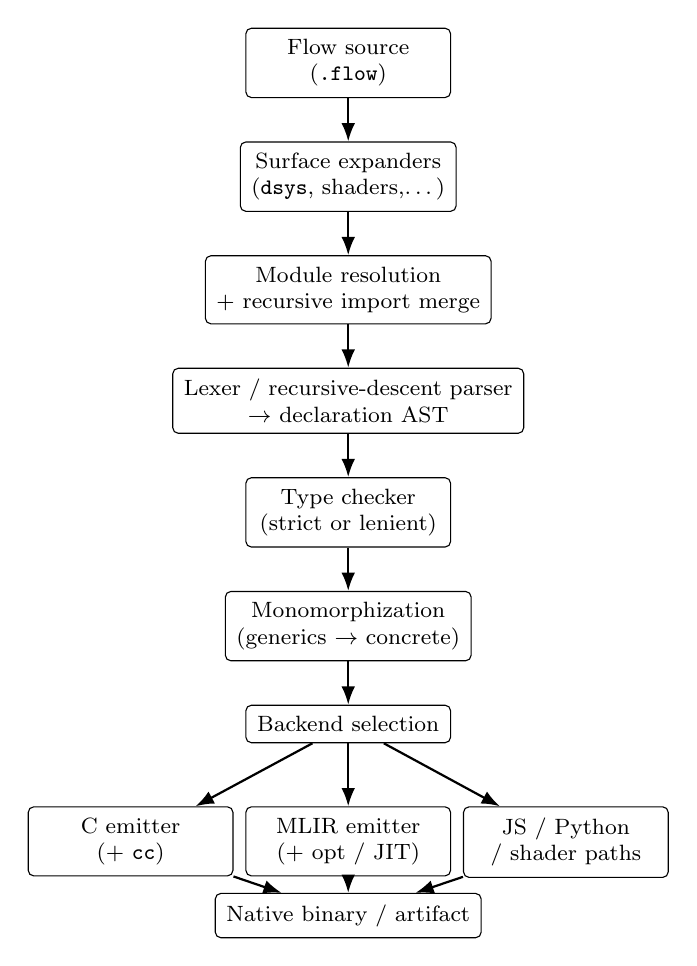
\begin{tikzpicture}[
  node distance=0.55cm and 0.9cm,
  box/.style={draw, rounded corners=2pt, align=center,
              font=\footnotesize, inner sep=4pt, minimum width=2.6cm},
  arr/.style={-{Latex}, thick}
]
\node[box] (src) {Flow source\\(\texttt{.flow})};
\node[box, below=of src] (exp) {Surface expanders\\(\texttt{dsys}, shaders,\ldots)};
\node[box, below=of exp] (mod) {Module resolution\\+ recursive import merge};
\node[box, below=of mod] (parse) {Lexer / recursive-descent parser\\$\to$ declaration AST};
\node[box, below=of parse] (tc) {Type checker\\(strict or lenient)};
\node[box, below=of tc] (mono) {Monomorphization\\(generics $\to$ concrete)};
\node[box, below=of mono] (be) {Backend selection};
\node[box, below left=0.8cm and 0.15cm of be] (c) {C emitter\\(+ \texttt{cc})};
\node[box, below=0.8cm of be] (mlir) {MLIR emitter\\(+ opt / JIT)};
\node[box, below right=0.8cm and 0.15cm of be] (other) {JS / Python\\/ shader paths};
\node[box, below=1.9cm of be] (bin) {Native binary / artifact};

\draw[arr] (src) -- (exp);
\draw[arr] (exp) -- (mod);
\draw[arr] (mod) -- (parse);
\draw[arr] (parse) -- (tc);
\draw[arr] (tc) -- (mono);
\draw[arr] (mono) -- (be);
\draw[arr] (be) -- (c);
\draw[arr] (be) -- (mlir);
\draw[arr] (be) -- (other);
\draw[arr] (c) -- (bin);
\draw[arr] (mlir) -- (bin);
\draw[arr] (other) -- (bin);
\end{tikzpicture}
\caption{Production Flow compilation pipeline. Surface expanders rewrite domain
syntax into core Flow before parsing. Generics are eliminated by monomorphization
prior to backend emission. The portable default is C; MLIR and specialized paths
are opt-in.}
\label{fig:pipeline}
\end{figure}

\section{Production frontend}
\label{sec:frontend}

\subsection{Module resolution}
\label{sec:modules}

Compilation begins at a root file. The module resolver recursively loads
imports (\texttt{import "path.flow"}), tracks visited files to break cycles,
and merges exported symbols into a single declaration list for downstream
passes~\cite{flow-readme}. Visibility is export-based: symbols are module-private
by default.

Critically, resolution is also the hook point for surface dialects. Before a
file is handed to the parser, the resolver may:

\begin{itemize}[leftmargin=*]
  \item detect and expand dynamics DSL blocks (\texttt{dsys}, \texttt{sense},
        \texttt{ga evolve}, \texttt{closed}, \texttt{represent linear}, \ldots)
        into calls against \texttt{lib/stdlib/dynamics};
  \item recognize fill-shader modules (\texttt{shader fill}) and divert them
        to the shader compilation path (or install a host stub so corpus
        transpile checks remain well-defined).
\end{itemize}

This ordering---expand, then parse---preserves a single recursive-descent
grammar for the core language while still allowing domain-shaped authoring.

\subsection{Lexer and parser}
\label{sec:parser}

The production lexer/parser (\texttt{parser.py}) builds a typed AST of
declarations and statements: functions, structs, effects, capabilities,
enums, traits/impls, constants, and the usual structured control flow
(\texttt{if}/\texttt{while}/\texttt{for \ldots\ in \ldots\ to \ldots},
\texttt{match}, \texttt{handle}).

Syntactic priorities of the living language include:

\begin{itemize}[leftmargin=*]
  \item explicit mutability (\texttt{let} vs.\ \texttt{let mut});
  \item explicit types on bindings and signatures;
  \item algebraic effect and capability declarations;
  \item FFI via \texttt{extern \{ \ldots \}} blocks;
  \item postfix chaining sufficient for systems libraries
        (indexing, field access, method calls).
\end{itemize}

\subsection{Type checking}
\label{sec:types}

The \texttt{TypeChecker} walks the merged declaration list under strict mode
by default (lenient mode demotes errors to warnings for transitional
corpora). Checking covers name resolution, arity, return consistency, and the
bulk of structural typing obligations expected of a C-emitting systems
language. The checker is a semantic gate before monomorphization: generics
remain in the AST until their uses are known.

\subsection{Monomorphization}
\label{sec:mono}

Flow generics are compiled by specialization, in the style of Rust's
monomorphization rather than Java-style erasure~\cite{flow-mono}. A generic
function or struct
\begin{lstlisting}
struct Option<T> { has_value: bool, value: T }
function identity<T>(x: T) -> T { return x }
\end{lstlisting}
is replaced, for each concrete instantiation site, by specialized clones
(\texttt{Option\_i32}, \texttt{identity\_i32}, \ldots). The trade-off is the
usual one: zero runtime dispatch cost and full static typing, at the expense
of code size. After this pass, backends may assume a monomorphic program.

\subsection{Mode guards}
\label{sec:guards}

Declarations may carry attributes that restrict them to particular execution
modes (\texttt{@only(jit)}, \texttt{@guard(c)}, hot-reload, \ldots). The
transpiler filters the declaration list according to the active backend and
CLI flags before emission, allowing a single source file to contain compile-time
and JIT-only variants without polluting the default binary.

\section{The portable C backend}
\label{sec:cbackend}

\subsection{Translation strategy}

The C generator (\texttt{c\_generator.py}) is the workhorse backend. It emits a
single translation unit (or a small set of units linked with runtime objects)
that a host \texttt{cc} can compile. Types map in the obvious way
(\texttt{i32}$\to$\texttt{int32\_t}, \texttt{f64}$\to$\texttt{double},
\texttt{ptr<T>}$\to$\texttt{T*}, structs to C structs, arrays to C arrays or
explicit buffers depending on shape).

Control flow lowers to C structured statements. Closures and higher-order
patterns that the language admits are compiled with explicit environment
representations where needed; the generator tracks nesting depth relative to
\texttt{handle} blocks so that escaping closures do not accidentally capture
transient handler state.

\subsection{Algebraic effects as vtables}
\label{sec:effects}

Flow's algebraic effects are the clearest linguistic differentiator relative to
C, Rust, Zig, and Mojo in the project's own comparison notes~\cite{flow-cmp}.
The C lowering is deliberately simple and ABI-shaped:

\begin{enumerate}[leftmargin=*]
  \item Each \texttt{effect E \{ op(\ldots) -> T, \ldots \}} becomes a C
        handler struct of function pointers (a vtable) plus a
        thread-oriented current-handler pointer.
  \item Each capability supplies concrete function implementations and a
        static vtable instance.
  \item A \texttt{handle E with Cap \{ \ldots \}} block saves the previous
        handler pointer, installs \texttt{Cap}'s vtable, executes the body,
        and restores the previous handler on exit (including nested handles).
  \item Effect operations compile to calls through the current handler; absent
        a handler, operations degrade to defined no-ops / zero returns rather
        than aborting---a pragmatic choice for demos and partial stacks.
\end{enumerate}

\begin{remark}[Tail-resumptive MVP]
The shipped effect system is \emph{tail-resumptive}: operations return to the
call site. There is no general delimited continuation, fiber scheduler, or
work-stealing runtime in the default lowering. Asynchronous APIs are therefore
modelled as effects with simulated or blocking capabilities, not as
\texttt{async}/\texttt{await} desugaring~\cite{flow-async}.
\end{remark}

This design keeps effectful Flow programs readable as ordinary C with an
explicit capability ABI, and makes handler swapping (production vs.\ test
backends) a matter of installing different vtables around the same call
graph~\cite{flow-effects}.

\subsection{Linking and runtimes}

Native features beyond ISO C---macOS/Linux graphics, Metal GPU memory, audio
device I/O, HTTP natives in registry packages---are linked as separate runtime
objects. The CLI selects which runtime objects to include based on imports and
command mode (\texttt{flow run}, \texttt{flow gfx}, \texttt{flow audio},
\ldots). The architectural invariant is that the \emph{language} backend remains
C; platform capability arrives as libraries, not as a second IR.

\section{Secondary backends and special paths}
\label{sec:secondary}

\subsection{MLIR / LLVM}

An MLIR generator lowers Flow ASTs to MLIR dialects (structured control flow,
memrefs, optional GPU dialect emission). Optimizations may be applied via
\texttt{mlir-opt}; JIT and hot-reload paths compile through LLVM tooling when
present. This path is important for experimentation and GPU dialect work, but
it is not the portability baseline.

\subsection{WebAssembly}

WASM is obtained by composing the C backend with Emscripten
(\texttt{emcc})~\cite{flow-wasm}:
\[
\text{Flow} \xrightarrow{\text{C backend}} \text{C}
  \xrightarrow{\text{emcc}} \text{.wasm + JS glue}.
\]
There is no Flow-in-WASM self-hosted toolchain; browser delivery reuses the
same portable C semantics as native builds.

\subsection{Fill shaders}

Fill-shader modules are a separate surface language compiled by
\texttt{shader\_codegen} / \texttt{./flow shader} to Metal fragment entry
points. They are intentionally not forced through the host Flow C pipeline as
ordinary functions; the module resolver isolates them so the core language does
not absorb shading grammar.

\subsection{Automatic differentiation}
\label{sec:ad}

Forward-mode AD ships as library dual numbers; reverse-mode helpers and
external gradient codegen tools exist as prototypes~\cite{flow-ad}. They are
\emph{not} currently a mandatory compiler IR pass. Architecturally this matters:
AD can deepen into a transformation pass once a stable typed IR and mutation
story for tapes exist; until then, the compiler treats AD as library and
tooling layered on the same AST/C pipeline.

\section{Surface languages as architectural components}
\label{sec:surfaces}

\subsection{Dynamics DSL (\texttt{dsys})}

The dynamics surface lets authors declare linear plants, horizons, sensing
predicates (controllability, spectral radius), genetic-algorithm gain search,
and closed-loop certificates without writing matrix boilerplate by hand.
Expansion injects setup code into \texttt{main} and binds analysis results as
ordinary locals~\cite{flow-dsys}. Continuous plants are Euler-discretized for
the present analysis envelope (notably small SISO LTI systems).

\begin{lstlisting}
dsys plant {
  discrete  dt 0.1  n 2 m 1 p 1
  A 1.0 0.1 0.0 1.0
  B 0.0 0.1
  C 1.0 0.0
}
sense on plant { controllable -> ok  spectral -> rho }
\end{lstlisting}

The architectural claim is not that the expander is a full hybrid-systems
compiler; it is that \emph{domain syntax hooks at resolve-time} are the
supported extension mechanism while the core grammar and C backend remain
stable.

\subsection{Evolution-oriented core syntax}

Beyond \texttt{dsys}, the language vision includes \texttt{flow} blocks with
\texttt{evolves as} dynamics and related timing/constraint forms. Where
implemented, these participate in the same resolve/parse/check/emit chain; where
still aspirational, they are tracked as roadmap work rather than silent
compiler magic~\cite{flow-vision}.

\section{Self-hosting: Stage-A \texttt{flowc}}
\label{sec:selfhost}

\subsection{Motivation}

Long-term, Flow aims to retire Python from the compile critical path: dogfooding,
a single toolchain story for users, and a subset forced by systems needs rather
than by host-language convenience~\cite{flow-selfhost}. Tooling (wiki build, some
LSP glue, benches) may remain Python longer; compilation should not.

\subsection{Stage-A modules}

\texttt{flowc} is structured as cooperating Flow modules with an index-based
AST arena (children and sibling chains stored as integer indices into a node
buffer---friendly to C emission and explicit memory management):

\begin{center}
\begin{tabular}{@{}llp{7.2cm}@{}}
\toprule
Module & File & Role \\
\midrule
\texttt{token}/\texttt{lexer} & \texttt{token.flow}, \texttt{lexer.flow} & Lexical analysis \\
\texttt{ast} & \texttt{ast.flow} & Tagged AST arena \\
\texttt{parser} & \texttt{parser.flow} & Recursive-descent subset parser \\
\texttt{typecheck} & \texttt{typecheck.flow} & Lightweight name/semantic checks \\
\texttt{resolve} & \texttt{resolve.flow} & Multi-file import + bundle emit \\
\texttt{cgen} & \texttt{cgen.flow} & Stage-A AST$\to$C buffer emitter \\
\texttt{jsgen}/\texttt{fmt} & \texttt{jsgen.flow}, \texttt{fmt.flow} & JS / pretty-print emitters \\
\texttt{driver}/\texttt{main} & \texttt{driver.flow}, \texttt{main.flow} & CLI / smoke / env-gated emit \\
\bottomrule
\end{tabular}
\end{center}

\subsection{Bootstrap ladder}

The classical ladder is instantiated concretely:

\begin{enumerate}[leftmargin=*]
  \item \textbf{Gen0.} The Python host compiles \texttt{compiler/src/*.flow}
        to C objects and links a driver (\texttt{flowc\_frontend.o} plus C or
        Flow driver).
  \item \textbf{Gen1.} That driver re-emits the frontend sources to
        \texttt{flowc\_frontend\_self.o}.
  \item \textbf{Gen2.} Gen1 re-emits again; object code is compared for
        fixed-point equality (\texttt{cmp} of \texttt{self.o} vs.\ \texttt{g2.o}),
        with smoke tests (e.g.\ fixture \texttt{stage\_a\_sum} exiting 45).
\end{enumerate}

\begin{proposition}[Partial self-host fixed point]
On the Stage-A subset and frontend module set exercised by the repository's
\texttt{stage\_a\_self\_emit\_g2} scripts, consecutive self-emits produce
byte-identical frontend objects under the documented toolchain. This does
\emph{not} yet imply that \texttt{flowc} compiles the full production language
or the Python compiler sources.
\end{proposition}

Bundle mode (\texttt{FLOWC\_BUNDLE=1}) resolves relative imports and
concatenates dependency C before the entry module, with optional
deps-first typechecking seeded by export sets---an MVP package story inside
Stage-A.

\subsection{Cutover plan (architectural)}

The documented plan proceeds by landing Stage-A in CI, closing the subset gap
until \texttt{flowc} can compile its own sources without escape hatches,
switching \texttt{./flow} to prefer the Flow driver, and only then retiring
Python from the hot path~\cite{flow-selfhost}. Dual-run parity on tiered example
corpora is the acceptance gate.

\section{Implementation scale and validation posture}
\label{sec:validation}

The repository maintains several validation layers that constrain architecture
changes:

\begin{itemize}[leftmargin=*]
  \item unit and corpus tests (\texttt{./flow test}, including strict tiers);
  \item example status tracking across hundreds of programs;
  \item Stage-A roundtrip and self-emit scripts;
  \item optional fuzz harnesses with crash regressions folded back as parser
        tests;
  \item microbenchmarks comparing Flow-emitted C to hand-written C under matched
        optimization flags (historically showing parity on dense linear algebra
        and Mandelbrot-style kernels when both lower to equivalent C)~\cite{flow-cmp}.
\end{itemize}

Architecturally, these layers encode a preference for \emph{executable
honesty}: documentation and papers should track what the pipeline actually
emits and runs.

\section{Related work}
\label{sec:related}

Flow's portable C backend sits in a lineage with languages that treat C as a
portable IR (early C++, historical paths in Zig, various research transpiler
languages), while its effect system relates to Eff, Koka, Frank, and Multicore
OCaml's effect handlers~\cite{bauer-pretnar,leijen-koka,lindley-frank,ocaml-effects}.
Monomorphization follows the specialization tradition of C++ templates and Rust
generics. MLIR as an optional path aligns with modern extensible compiler
infrastructure~\cite{mlir}. Self-hosting bootstraps are classical
(Pascal, GCC, Go, Rustc stages); Flow's contribution is not novelty of the
ladder shape but the concrete dual-host staging around a C-first systems
language with domain expanders.

Relative to MATLAB/Simulink and Modelica, Flow's dynamics surface is narrower
today (LTI seed) but aims at a single deployable artifact rather than a
model/code split~\cite{flow-cmp}. Relative to Mojo, Flow emphasizes effects and
portable C over Python-first ML runtime integration; relative to Rust, Flow
trades a borrow checker for effect capabilities and a simpler default ABI
story.

\section{Limitations}
\label{sec:limits}

\begin{enumerate}[leftmargin=*]
  \item \textbf{Dual host cost.} Until cutover, language bugs may require fixes
        in both Python and Flow-written frontends for overlapping subsets.
  \item \textbf{Effect expressiveness.} Tail-resumptive handlers exclude many
        classical effect patterns (coroutines, non-deterministic search) without
        further runtime work.
  \item \textbf{AD depth.} Library dual numbers and external grad tools are not
        yet a unified compiler AD pass.
  \item \textbf{Dynamics envelope.} The shipped \texttt{dsys} analysis path is
        intentionally small-dimensional; larger plants still use hand-written or
        stdlib numerical code.
  \item \textbf{Stage-A coverage.} Effects, full generics, and most production
        DSL surfaces remain outside \texttt{flowc}'s subset.
\end{enumerate}

\section{Conclusion}
\label{sec:conclusion}

The Flow compiler is best understood as a \emph{C-centred, dual-host}
architecture: a production Python pipeline that already supports a broad
language surface---including algebraic effects lowered to handler vtables,
monomorphized generics, and resolve-time domain expanders---and a Flow-written
Stage-A compiler that is climbing a classical self-hosting ladder toward
retiring Python from the compile path. Secondary backends (MLIR, WASM via
Emscripten, Metal shaders) specialize without displacing the portable default.

The architectural bets are deliberate: keep the core grammar stable; encode
capabilities as ABI; expand domain syntax before parsing; specialize generics
before emission; and treat self-hosting as an evidence-driven bootstrap with
fixed-point checks rather than a slogan. Future work follows directly from
those bets---closing the Stage-A subset gap, deepening effect runtimes beyond
tail-resumption, and optionally promoting AD and richer hybrid dynamics from
library/expander status into typed IR transformations---without abandoning the
portable C spine that makes Flow deployable with ordinary system toolchains.

\section*{Reproducibility}
\label{sec:repro}

The architecture described here corresponds to the open-source repository
\url{https://github.com/flooooooooooow/flow}. Representative commands:

\begin{lstlisting}[basicstyle=\ttfamily\scriptsize]
# Production path
./flow run examples/basics/hello_world.flow
./flow compile examples/effects/showcase.flow

# Stage-A roundtrip / self-host smokes (from repo root)
./compiler/scripts/roundtrip.sh
./compiler/scripts/stage_a_self_emit_g2.sh

# Dynamics surface
./flow run examples/dynamics/ga_dsys_syntax.flow
\end{lstlisting}

Primary documentation sources mirrored in this paper:
\texttt{compiler/README.md}, \texttt{docs/project/self-hosting.md},
\texttt{docs/language/dynamics-dsl.md}, \texttt{docs/effects-showcase.md},
\texttt{docs/library/autodiff.md}, and \texttt{docs/language/wasm.md}.

\begin{thebibliography}{99}

\bibitem{flow-vision}
Flow project.
\textit{VISION.md --- A programming language where the primary abstraction is
the evolution of systems through time}.
Flow repository documentation, 2026.

\bibitem{flow-readme}
Flow project.
\textit{README.md} and compiler module map.
\url{https://github.com/flooooooooooow/flow}, 2026.

\bibitem{flow-selfhost}
Flow project.
\textit{Self-Hosting Plan --- Rewrite the Compiler in Flow}.
\texttt{docs/project/self-hosting.md}, 2026.

\bibitem{flow-effects}
Flow project.
\textit{Effect System Showcase: One Service, Many Worlds}.
\texttt{docs/effects-showcase.md}, 2026.

\bibitem{flow-async}
Flow project.
\textit{Async via Effects}.
\texttt{docs/language/async-effects.md}, 2026.

\bibitem{flow-dsys}
Flow project.
\textit{Dynamics DSL (\texttt{dsys})}.
\texttt{docs/language/dynamics-dsl.md}, 2026.

\bibitem{flow-ad}
Flow project.
\textit{Autodiff}.
\texttt{docs/library/autodiff.md}, 2026.

\bibitem{flow-wasm}
Flow project.
\textit{WebAssembly (WASM) target}.
\texttt{docs/language/wasm.md}, 2026.

\bibitem{flow-cmp}
Flow project.
\textit{Flow vs C $\cdot$ Rust $\cdot$ Zig $\cdot$ Mojo}.
\texttt{docs/comparison.md}, 2026.

\bibitem{flow-mono}
Flow project.
\textit{Monomorphization pass} (\texttt{src/flow/monomorphize.py}), 2026.

\bibitem{bauer-pretnar}
A.~Bauer and M.~Pretnar.
Programming with algebraic effects and handlers.
\textit{Journal of Logical and Algebraic Methods in Programming}, 84(1):133--148, 2015.

\bibitem{leijen-koka}
D.~Leijen.
Koka: Programming with row polymorphic effect types.
\textit{MSFP}, 2014.

\bibitem{lindley-frank}
S.~Lindley, C.~McBride, and C.~McLaughlin.
Do be do be do (Frank).
\textit{POPL}, 2017.

\bibitem{ocaml-effects}
S.~Dolan, S.~Eliopoulos, D.~Hillerstr{\"o}m, A.~Madhavapeddy, K.~C.~Sivaramakrishnan, and L.~White.
Concurrent system programming with effect handlers.
\textit{TFP}, 2017.

\bibitem{mlir}
C.~Lattner et~al.
MLIR: Scaling compiler infrastructure for domain languages.
\textit{CGO}, 2021.

\end{thebibliography}

\end{document}
